\section{Code beispiele}

\subsection{Hello World}

\begin{lstlisting}[language = c]
#include <stdio.h>
int main()
{
    printf ("Hello World \n");
    return 0;
}
\end{lstlisting}

\subsection{Array Durchlaufen}

\subsubsection{1D}

\begin{lstlisting}[language = c]

int speicher[10];//Array definition

for(int i = 0;i < 10,i++)
{
    speicher[i] = 1;//Das Array wird mit 1 gefuellt
}
\end{lstlisting}

\subsubsection{mehrere Dimensionen}

\begin{lstlisting}[language = c]
int speicher[3][4] = {
    {0, 1, 2, 3},
    {4, 5, 6, 7},
    {8, 9, 10, 11}};//Array definition mit initialisierung
for(int i = 0;i < 3,i++)
{
    for(int j = 0; j < 4; j++)
    {
        speicher[i][j] = (i*4) + j;//Das Array von 0 bis 11 der reihe nach gefuellt.  
    }
}//Nach diesen for loops ist das Array gleich gebliben.
\end{lstlisting}

\subsection{Iterativ vs rekursiv}

Das Folgende Beispiel zeigt eine Implementation wo eine n-te Fibonacci Zahl bestimmt werden kann. Entweder iterativ oder rekursiv.\newline
Der Algorithmus : \[ f(1) = f(2) = 1 \newline f(n) = f(n-1) + f(n-2) \] wird verwendet.

\begin{lstlisting}[language = c]
#include <stdio.h>

unsigned int fibRek(unsigned int in);
unsigned int fibIt(unsigned int in);

int main()
{
    unsigned int input;
    int choose;

    scanf("%u",&input);
    printf("Iterativ oder rekursiv? (0 = rekursiv 1 = iterativ) \n ");
    scanf("%d",&choose);
    if(choose)
    {

        printf("Die %u te Fibonacci Zahl iterativ ist %u \n",input,fibIt(input));
        return 0;
    }
    printf("Die %u te Fibonacci  Zahl rekursiv ist %u  \n",input,fibRek(input));
    return 0;
}

unsigned int fibRek(unsigned int in)
{

    if(in == 2 || in == 1)
    {
        return 1;
    }
    return (fibRek(in-1) + fibRek(in-2));
}

unsigned int fibIt(unsigned int in)
{
    unsigned int out = 1;
    unsigned int outPrev = 0;

    for(int i = 1;i < in;i++)
    {
        out = out + outPrev;
        outPrev = out - outPrev;
    }

    return out;
}

\end{lstlisting}



\section{emotional support meme}

Für den Fall das während der Prüfung emotionaler Support gefragt ist ein meme:
\begin{center}
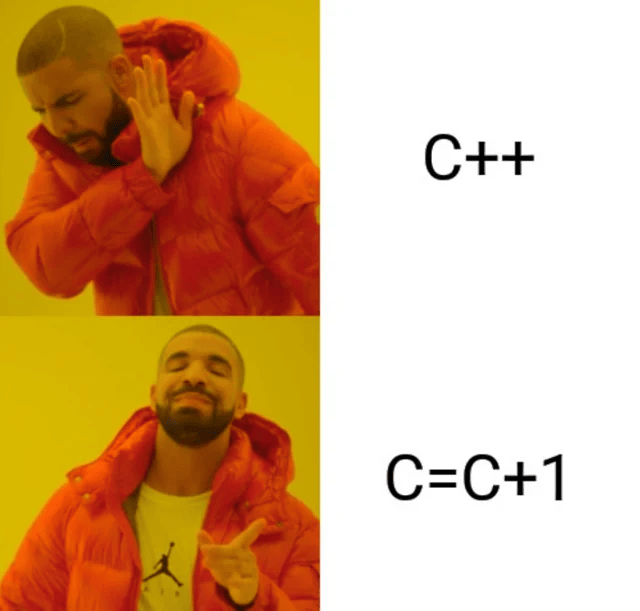
\includegraphics[width=0.5\columnwidth]{Pictures/emotional_support_meme.png}
    
\end{center}
